\begin{figure}[!h]                
	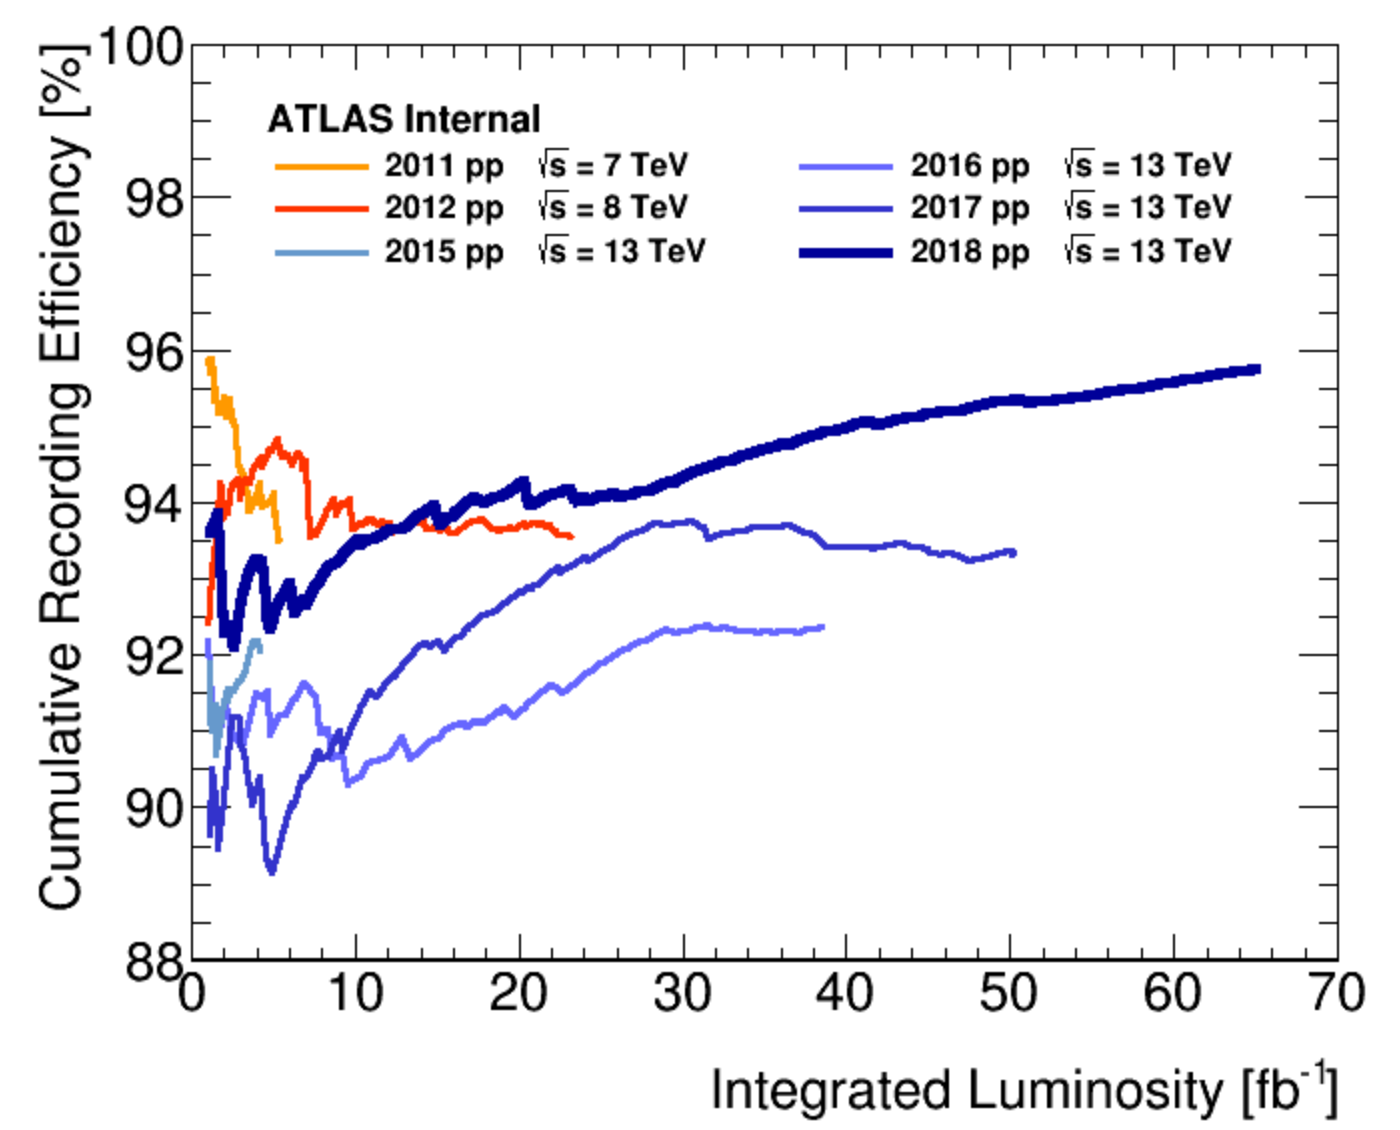
\includegraphics[width=0.6\textwidth]{Chapter2/recefficiency.png}
	\centering
	\begin{center}
		\caption{The ATLAS recording efficiency and luminosity \cite{Pontecorvo:2638061}}
		\label{Fig:recefficiency}            
	\end{center}
\end{figure}
\section{Object Reconstruction}
\label{sec:obj rec}
When the events are passed into the permanent storage, they are still in the format of raw data which contains only the information of hits (the spacepoints from the inner detector and muon spectrometer) and calorimeter energy towers (the energy deposited in the calorimeter cells). They need to go though the full reconstruction (offline reconstruction) to be interpreted into the objects with physical meanings as the SM particles like electrons or muons. The reconstruction will be based on the principles of interactions between detectors and particles: 
\\
\\1) Only charged particles leave tracks in the inner detector
\\
\\2) The charged particles shall deposit energy in the ECAL, and the light ones are stopped here.
\\
\\3) All the particles except for muons are supposed to be stopped in or before the HCAL.
\\
\\4) Only muons could reach the muon spectrometer. 
\\
\\After the reconstruction of all subjects, a further correction on energy scale (the peak of the energy pulse shape) is applied on both data and simulation samples to take in  the effect of energy loss from the radiation, the contamination from other objects, or the detector effect (like dark current, hot noise, or material inhomogeneities). The final procedure is to remove the overlapped objects by the priority defined by the analyses. 
\\
\\{\bf Primary Vertex $\&$ Tracks \cite{Aaboud:2017all}}
\\
\\A pattern recognition is performed in the SCT to find the helical trajectories with at least 3 spacepoints and $p_{T}>500MeV$ which are taken as the track seeds. A Kalman Filter algorithm is then performed to extend the track seeds to the pixel layers. To resolve the reconstruction ambiguity, a tracking score system is taken to reject the shared spacepoints or fake tracks. When a track is reconstructed with more hits and less ``holes'' (missing hits in some layers), it is given a higher score. The final tracks shall all have at least seven hits (three spacepoints from SCT and four hits from pixel). To complete the track reconstruction, the projection route from the outermost SCT spacepoint of a track passes through TRT, and the drift tubes within $10mm$ from the route are integrated into the track. Afterwards, one addition track reconstruction (outside-in) from TRT is performed to recover the tracks from the late decay or photon conversion. The unused TRT segments are then rematched to the SCT and pixel hit remanent.   
\\
\\The crossing points of tracks near the LHC pipelines are then assumed to be where the interactions happen, which are called ``vertices''. The vertex associated with the highest $p_{T}^2$ sum is then defined as the primary vertex. All the reconstructed objects should origin from the primary vertex which is verified by $d_{0}$ and $d_z$, the distances between the object and the primary vertex in the x-y plane and the z-axis, or they are taken as ``minimum bias'' background.  
\\
\\{\bf Electrons}
\\
\\Electrons are charged light particles, so they leave tracks in the inner detector and energy clusters in the ECAL. The two types of signature are combined and testified to reconstruct electrons.
\\
\\The first stage of the reconstruction is to build the energy cluster as an electron seed \cite{ATLAS-CONF-2016-024,ATL-LARG-PUB-2008-002}. A window of $3 \times 5$ ECAL layer-2 cells (corresponding to $0.075 \times 0.125$ in $\Delta \eta \times \Delta \phi$) is used to scans through ECAL layer-2 to find the electron seeds. If the transverse energy sum ($E_{T}$) inside the window is above $2.5GeV$, the cells inside this window are selected, and the electron position is defined as the energy weighted $\eta$ and $\phi$ (barycentre) of this window. Then, this window is extended along the $R$-direction to sum over the energy in other layers with the adjusted window size (detailed in ~\cite{}). The cells taken in the cluster are then removed to avoid the duplication into other electrons. With the estimation from $Z\to ee$ simulation sample, this algorithm has the electron reconstruction efficiency of $95\%$ ($>99\%$) for $E_{T}\sim7GeV$ ($E_{T}>15GeV$).
\\
\\The reconstruction of tracks associated to electrons is performed independently from the mentioned reconstruction . A track seed of $p_{T}>1GeV$ is firstly reconstructed with three spacepoints from the SCT layers . Then, based on the pion hypothesis (pion energy loss pattern in the ID materials), it is verified by whether this track seed can be extended to pixel with four hits and matched to a calorimeter cluster. If it fails, the electron hypothesis is applied for the same verification. The hits from both hypotheses are then fitted using ``ATLAS Global $\chi^{2}$ Track Fitter''\cite{Cornelissen:2008zza} into tracks, and the tracks failing the pion track hypothesis are then tested again with electron hypothesis. The tracks passing the electron hypothesis are then taken as potential electron tracks. This algorithm is also integrated in the standard track reconstruction with the least interference.
\\
\\The track and cluster are then associated with a loose $\Delta R$ matching which considers the electron bremsstrahlung and the number of hits in the inner detector. The matched track-cluster pairs are then refitted with optimised ``Gaussian Sum Filter'' (GSF) \cite{ATLAS-CONF-2012-047} to take non-linear bremsstrahlung into account. 
\\
\\To have further separation between signal-like and background-like electrons, the electron identification is then performed on $Z \rightarrow ee$ (signal) and dijet (background) MC samples. It is a multi-variable analysis (MVA) based on the likelihood discriminant defined as:
\\
\begin{equation}
d_{\mathcal{L}}=\frac{\mathcal{L}_{S}}{\mathcal{L}_{S}+\mathcal{L}_{B}}    
\quad \text{ and } \quad
\mathcal{L}_{S(B)}(\vec{x})=\prod_{i = 1}^{n}P^{i}_{S(b)}(x^{i})
\end{equation}
where $P^{i}_{S(b)}(x^{i})$ is the probability density function for a specific input variable $x^{i}$, and $\vec{x}$ is the vector formed by them in the likelihood phase space of all input variables (all the input variables could be found in \cite{}). Three working points are therefore defined by $d_{\mathcal{L}}$: $Tight$, $Medium$ and $Loose$\footnote{$Tight$ selected electrons are the subset of $Medium$, and $Medium$ is the subset of $Loose$}. The signal efficiency from this selection process is as a function of electron $E_{T}$, and the plateau of efficiency could be reached at $E_{T}~70GeV$ for $~97\%$ ($~95\%$) [$91\%$] on $Loose$ ($Medium$) [$Tight$] working point. 
\\
\\In addition to the reconstruction quality, the electrons are also required to be ``isolated'' from all the other tracker and calorimeter signatures, because of the concern that the nearby detector activities might affect the electron measurement. The isolation is defined in two ways: 
\begin{itemize}
	\item the calorimeter isolation ($Iso^{E_{T}}$): it is defined as the cluster $E_{T}$ sum within a cone with $R=0.2(0.3)$ centred at the reconstructed electron inside which a central cluster subset in a rectangle of $0.125 \times 0.175$ ($\Delta \eta \times \Delta \phi$) is subtracted.
	\item the track isolation ($Iso^{p_{T}}$): it is defined as the $p_{T}$ sum of tracks from primary vertext within a cone of $R=min(0.2(0.3), 10GeV/E^{e}_{T})$ centred at the electron but without the electron associated tracks.  
\end{itemize}
The isolation discriminant is then applied as $Iso^{E_{T}}/E_{T}$ or $Iso^{p_T}/p_{T}$. The recommendation working points on the discriminant are given as a function of $E^{e}_{T}$ or fixed cut which are summarised with the muon isolation working points in Tab. \ref{Tab:iso}. 
\\
\\{\bf Muons \cite{Herde:2059849}}
\\
\\Muons are heavy enough to travel through the calorimeter and reach the MS, but the reconstruction is mainly based on the tracks in the inner detector and the MS. 
\\
\\The MS track segments are firstly built from the hits within each MS module, but the reconstruction coordinates are different in each subsystem: the MDT reconstruction is on the coordinate of the toroid magnetic bending plane, while the RPC and TCG have the coordinate orthogonal to it, and the CSC is only using the detector $\eta$-$\phi$ coordinate. A loose criteria is applied in the segment building algorithm to verify the compatibility to a full track. Then, the segments in the middle layer of the MS are taken as the track seed and extended to the inner and outer layers. If two segments could be fitted with enough hits by matching from their relative position and angle, they are integrated into the same track. The exception is in the transition region between the barrel and endcap, and a standalone and good-quality segment could be kept as a single track.  
\\
\\An overlap removal is afterwards applied to remove the shared hits in the tracks with poor fitting quality, but they could still be kept only if the fitting criterion is fulfilled. Two tracks could share maximally two hits in the inner two layers and have no same hit in the outer layer for the concern of close-by muons. 
\\
\\The hits along the tracks are then taken into the global $\chi^{2}$ fitting. The hits with great deviation from the fitted MS trajectory are removed, and the fit is applied again to derive the new track. If there are hits not included in the track but within the allowed deviation from the track, they are also taken into the track, and the fitting is repeated. 
\\
\\The final MS tracks are taken as the seed to match to the inner detector tracks to reconstruct the combined muons. A further global fitting is conducted to extrapolate the muons with the flexibility to add in or remove the MS hits to improve the fitting quality with the ID tracks. The primary algorithm in the fitting is performed outside-in from the MS to the inner detector, and a complementary algorithm of inside-out is also applied to guarantee the robustness of the reconstruction. For the muons outside of the inner detector coverage ($2.5<|\eta|<2.7$), they can be reconstructed from only MS tracks, but the criteria are more stringent. 
\\
\\Similar to electrons, muons also have the identification procedure with three parameters: $q/p$ significance (the ratio of charge and momentum measured in the ID and MS over the quadrature sum of their uncertainty), $\rho'$ (the ratio of momentum difference between the ID and MS measurements over the combined measurement) and the normalised combined track fit, $\chi^2$. The working points for the muons identification have the definition individually as below:
\begin{itemize}
	\item $Medium$ muons: they are defined within the range of $0.1<|\eta|<2.5$ with at least two layers of $\geq 3$ hits. If it is within the range, $0.1<|\eta|$, it is allowed to have hits in only one layer, but there shall be no hole in the MS track reconstruction. As the muons go beyond the coverage of the inner detector (i.e. $2.5<|\eta|<2.7$), they shall have the MS tracks reconstructed from all three layers. An extra requirement of $q/g$ significance above seven is also applied on this muon quality. 
	\item $Loose$ muons: those muons are defined with the most loose requirement. They are generally $Medium$ muons, but the selection is loosen for the range of $|\eta|<0.1$ due to the missing coverage of the MS (where a gap is present for the service of the ID and calorimeter). When an ID track is found within this range and matched to a calorimeter cluster which is identified as a deposit by ``minimum-ionization'' particles, they are also accepted as loose muons to recover the reconstruction efficiency. 
	\item $Tight$ muons: all of them must have the tracks reconstructed from two layers in the MS (either MDT or CSC) with $Medium$ muon hit selection. To enhance the purity of muons, a further requirement on the ID to MS track fitting is also added into the selection for $\chi^2<8$. An addition two-dimension cut on $q/g$ significance and $\rho'$ is also applied to improve the background rejection for muons with $p_{T}<20GeV$.
\end{itemize}
For the muon isolation, the definition is similar to the electron ones, but they have different working points. The recommended working points for electrons and muons are shown in tab. \ref{Tab:iso}.

\begin{table}[h]
	\caption{Electron/Muon Isolation Working Points}
	\renewcommand{\arraystretch}{1.5}
	\centering
	\begin{adjustbox}{center}
		\begin{tabular}{|c | c | c | c | c |}
			\hline
			\hline
			{\bf Working Point} &{\bf Object} &{\bf Calo Iso}                   &{\bf Track Iso}  &{Combined Iso} \\
			\hline
			LoseeTrackOnly      &all leptons  &-                                      &$99\%$                 &$99\%$               \\
			\hline
			Loose               &all leptons  &\multicolumn{2}{|c|}{$99\%$}                                   &$99\%$               \\
			\hline
			Gradient            &all leptons  &\multicolumn{2}{|c|}{$\epsilon=(0.1143*p_{T}[GeV]+92.14)\%$}   & \shortstack{\footnotesize{$\epsilon(25GeV)=90\%$} \\  \footnotesize{$\epsilon(60GeV)=99\%$}}\\       
			\hline
			GradientLoose       &all leptons  &\multicolumn{2}{|c|}{$\epsilon=(0.057*p_{T}[GeV]+95.57)\%$}   & \shortstack{\footnotesize{$\epsilon(25GeV)=95\%$} \\  \footnotesize{$\epsilon(60GeV)=99\%$}}\\
			\hline
			FixedCutTight       &Electrons  &\footnotesize{topoetcone20/pT<0.06}                 &\footnotesize{ptvarcone20/pT<0.06}  &-               \\
			\hline
			FixedCutTight       &Muons  &\footnotesize{topoetcone20/pT<0.06}                 &\footnotesize{ptvarcone30/pT<0.06}  &-               \\
			\hline
			\footnotesize{FixedCutTightTrackOnly}      &Electrons     &-                 &\footnotesize{ptvarcone20/pT<0.06}  &-               \\
			\hline
			\footnotesize{FixedCutTightTrackOnly}      &Muons      &-                 & \footnotesize{ptvarcone30/pT<0.06}  &-               \\
			\hline
			FixedCutLoose        &Electrons  & \footnotesize{topoetcone20/pT < 0.2} & \footnotesize{ptvarcone20/pT < 0.15}  & - \\
			\hline
			FixedCutLoose        &Muons  & \footnotesize{topoetcone20/pT < 0.3} & \footnotesize{ptvarcone30/pT < 0.15}  & - \\
			\hline
			\footnotesize{FixedCutHighPtCaloOnly} & Electrons &  \footnotesize{topoetcone20} < 3.5 GeV & - &-\\
			\hline
			\footnotesize{FixedCutHighPtTrackOnly} & Muons &  - &  \footnotesize{ptcone20} < 1.25 GeV  &-\\
			\hline
		\end{tabular}
	\end{adjustbox}
	\label{Tab:iso}
\end{table}
\noindent
{\bf Jets}
\\
\\When quarks or gluons are travelling in the space, they went through the process called ``fragmentation'' or ``hadronization'' for ``color-confinement'' of QCD. This leads to the multiplication of quarks, gluons (i.e. partons) or even leptons and photons, and they eventually form the bound states as hadrons leaving complicated signatures in the detector. One quark from a collision might leave more than one hundred tracks in the inner detector and several clusters in the calorimeter, and jets are defined as the ensemble of those signatures. To properly collect those tracks and calorimeter clusters into the same jets, the reconstruction algorithm is designed to ensure the infrared safety and collinear safety. The infrared safety means that 
the soft radiation from hadronic objects in a jet would not change the jet width or orientation, while the collinear safety indicates that the nearby particles with higher $p_{T}$ in the collinear direction of the splitted parton would not affect the jet reconstruction. To achieve both of the two requirements, the jet reconstruction algorithm\cite{Atkin:2015msa} employs the following two parameters for the jet definition: 
\begin{equation}
d_{ij}=min((p_{t}^{i})^{a},(p_{t}^{j})^{a})\times \frac{R_{ij}^{2}}{R}
\quad \text{ with } \quad
d_{iB}=(p_{t}^{i})^{a}
\end{equation}
where $p_{t}^{i}$ and $p_{t}^{j}$ are $p_{T}$ of $i$th and $j$th entities which could be calorimeter clusters (a patch of energetic cells in the calorimeter), tracks, or the truth particles from the simulation, $R_{ij}$ is the distance between them, and R is the parameter to customize the algorithm for performance (i.e. cone size), while $a$ corresponds to three algorithms which are sensitive to different jet properties. $a=-2$ is for $anti-k_{t}$ algorithm, and it has the advantage for better stability of jet structure during reconstruction with high sensitivity to hard objects and ignorance for the jet substructure as well as pile-up events. $a=0$ and $a=-2$ are used for Cambridge-Aachen algorithm and $k_{t}$ algorithm respectively which are more sensitive to jet substructure but with high dependence on pile-up events and soft objects. When $d_{ij}<d_{iB}$, the $i^{th}$ and $j^{th}$ objects are merged into the same cluster with the position defined as their barycentre. If no new pair could be found meeting this condition, the cluster is then defined as a jet. To make further 
\\
\\For the jets in the ATLAS experiment, $anti-k_{t}$ algorithm is preferred with $R=0.4$ and $R=1.0$ with the inputs objects. $R=1.0$ is for the scenario that two jets are close to each other, and $R=0.4$ could not have the separation power to distinguish each of them. The input entities for jet reconstruction is the ECAL topo clusters in the range of $|\eta|<4.9$, the calorimeter coverage, with energy $2\sigma$ above the quadrature sum of pile-up events and electronic noise, while the seeding cluster to initiate the clustering has higher requirement of $4\sigma$. The hadronic energy deposit from HCAL is added to the ECAL clusters through ``local cell weighting'' (LCW)\cite{Barillari:1112035} which is to calibrate the jet energy scale by the MC simulation and the data from the single particle test beam. The final reconstructed jets are then used in analyses after the selection of ``jet vertex tagger'' (JVT)\cite{ATLAS-CONF-2014-018} to guarantee that they originate from the primary vertex. 
\\
\\{\bf b-Tagging\cite{ATL-PHYS-PUB-2015-022}}
\\
\\b quarks take over the greatest branch ratio of Higgs boson decay, and it is always the decay product of top quarks(BR($t \rightarrow bW$)=$100\%$) which is the major background for most ATLAS analyses. Therefore, how to recognize the jets from b quarks is an important task for physics purposes.
\\
\\Different from the signatures other stable SM particles leave in the detector, b-quarks have a ``pseudo-short'' lifetime, so the jets of b-quarks have a displaced vertex several $mm$ away from the primary vertex. The b-jet identification depends on this property and the b-quark decay chain. The following three algorithms are used:
\begin{itemize}
	\item {\bf Impact Parameter based Algorithms}: given their displaced vertex, b-jet associated tracks should tend to have a greater impact parameter in both transverse and longitudinal directions. The impact parameters are used as inputs for the probability density function of the ratio of possibility of b-quark and light-flavour quark hypotheses, which are then combined into a single log likelihood ratio discriminant (LLR).
	\item {\bf Secondary Vertex Finding Algorithm}: to reconstruct the secondary vertex, the first step is to find the vertices with only two tracks. The tracks from the vertices far from the primary vertex, they are rejected. They might be from long-lived hadron decay (like kaon), photon conversion or hadronic interaction with materials.  The secondary vertex is then reconstructed from the survived tracks with outlier tracks removed
	\item {\bf Decay Chain Multi-Vertex Algorithm}: this algorithm is also called ``jet finder''. Its purpose is to find the full chain of ``$PV \rightarrow b \rightarrow c$''. A Kalman filter is applied to link the vertices to approximate the trajectories of this jet with which the vertices of b- and c-quarks could be resolved even with only one-track link.  
\end{itemize}
\noindent
The output of those algorithms are then given to a multi-variable analysis (MVA) of Boosted Decision Tree for the final discriminant. It is trained with the sample of $t\bar{t}$ which contains b-jets and the background composed of $10\%$ c-jets and $90\%$ other light-flavour jets. The final outcome, BDT score, is then applied as a simple cut to select b-jets, and the suggested working points are shown in tab. \ref{Tab:b-tag}

\begin{table}[h]
	\caption{b-Tagging Working Points}
	\renewcommand{\arraystretch}{1.5}
	\centering
	\begin{adjustbox}{center}
		\begin{tabular}{|c | c | c | c |}
			\hline
			\hline
			{\bf Cut Value}    & {\bf b-jet Efficiency[$\%$]}  & {\bf c-jet Rejetction} & {\bf light-flavour-jet Rejection}\\
			0.4496 & 60 & 21 & 1900 \\
			-0.0436& 70 & 8.1& 440 \\
			-0.4434& 77 & 4.5&  140 \\
			-0.7787& 85 & 2.6&  28 \\
			\hline
		\end{tabular}
	\end{adjustbox}
	\label{Tab:b-tag}
\end{table}		
\noindent
{\bf Missing Transverse Energy (MET)}
\\
\\The design of the ATLAS detector utilizes electromagnetic and hadronic interactions to capture particles. If particles are only involved in weak interactions, they leave no signatures in the detector like neutrinos or some new particles predicted by BSM theories. In this case, the only way to measure their energy is via the momentum conservation. 
\\
\\When two protons collide into each other in the LHC, both of them have no momentum on the transverse plane, so the transverse momentum sum of collision products is supposed to be zero. Therefore, the definition for sum of transverse momentum from invisible particles could be presented as:
\begin{equation}
\vec{E}_{T}^{miss} = \sum_{\text{visible objects}} -\vec{p}_{T}^{i}
\end{equation}
where $E_{T}^{miss}$ is supposed to be called missing transverse momentum, but it is called ``missing transverse energy'' out of historical reason. The explicit form is:
\begin{equation}
\vec{E}_{T}^{miss} = -(\sum \vec{p}_{T}^{e} +\sum \vec{p}_{T}^{\mu} +\sum \vec{p}_{T}^{\gamma} +\sum \vec{p}_{T}^{jet} +\sum \vec{p}_{T}^{\tau}+\sum \vec{p}_{T}^{soft})
\end{equation}
with $p_{T}$ contributed from different objects passing loose selection. Even though tau, $\tau$, and photon, $\gamma$, are not used in the analysis, they are still reconstructed and applied in $\met$ estimation.  The last term is referred to the detector soft signatures which are not used in the reconstruction of any objects. They could be either from tracks (track soft term, TST) or clusters (cluster soft term, CST). The track soft term considers only the remaining tracks from the primary vertex, so it has lower dependence on the pile-up events, while it cannot deal with the contribution from neutral objects which, instead, could be recovered by the CST. In ATLAS Run2 analyses, TST is preferred, because it delivers smaller uncertainty with the high pile-ups. As $E^{T}_{miss}$ is only calculated on the transverse plan, it has no $\eta$ information. 

\section{Simulation}
\label{sec:simulation}
For the two analyses in this thesis, the SM background estimation comes from the Monte Carlo simulation. It is performed in a couple of steps: event generation $\rightarrow$ event overlapping with ``minimum bias'' (MB) events $\rightarrow$  detector response simulation $\rightarrow$ digitization $\rightarrow$ physical object reconstruction $\rightarrow$ physics analysis.
\\
\\Event generation is through the generators designed by theorist with the input of theoretical parameters for the interactions: $pp(\rightarrow X)\rightarrow Y$. $X$ is the medium state particle with short lifetime, and it will eventually decay to Y as the final stable particles leaving signatures in the detector with the kinematic properties assigned by the event generator. The total cross section of the interaction will then be evaluated by this equation\cite{Plehn:2008zs}: 
\begin{equation}
\sigma_{pp\rightarrow Y} = \sum_{a,b} \int dx_{1}dx_{2}f_{a}(x_{1},\mu_{1})f_{b}(x_{2},\mu_{2})\hat{\sigma}_{a,b\rightarrow X}(x_{1},x_{2},\mu_{R})
\end{equation}
with a,b as the flavours for the proton partons (quark or gluon) involved in the interaction, and $x_{1}$ and $x_{2}$ are the momentum fraction of the partons relative to the whole proton, $\hat{\sigma}_{a,b\rightarrow X}$ is the cross-section calculated perturbatively of the process, $a,b\rightarrow X$, and $f_{a}$, $f_{b}$ are the parton distribution function (p.d.f.) for the corresponding parton flavours which give the possibility of the momentum transfer from partons to the output stable particles. $\mu_{1}$, $\mu_{2}$, and $\mu_{R}$ are the factorization factors which decide how the p.d.f. evolves. 
\\
\\For the ATLAS simulation, two processes are simulated in one event: pile-ups, $pp\rightarrow jj$, and hard-scattering, $pp(\rightarrow X)\rightarrow Y$ with $X$ and $Y$ as the particles of interests. Generally, hard-scattering is generated with a specific generator which can give the best accuracy of simulation, and the events are then passed to $PYTHIA8$\cite{Sjostrand:2008vc,Sjostrand:2007gs} for the generation of pile-up events and the hadronizaton of the hadronic objects. 
\\
\\The next step is to simulate the interaction between the particles and the detector. The detector is described by $GEANT4$\cite{Agostinelli:2002hh} with the input parameters like materials and logical volumes. The detector description is then stored in the ATLAS Geometry database which has low flexibility to change the content, while an additional database, COOL, is used to keep the information changed with time like dead channels and LAr high voltage settings. The particles are then parametrized to interact with the detector, which gives the digitalised output of raw data objects like tracks and calorimeter clusters. After the same physical object reconstruction from the detector signatures as data, the simulation samples are ready for the physical analyses in the data format called ``analysis object data'' (AOD). The full procedure could be seen in the diagram of Fig. \ref{Fig:simulation}
\begin{figure}[!h]                
	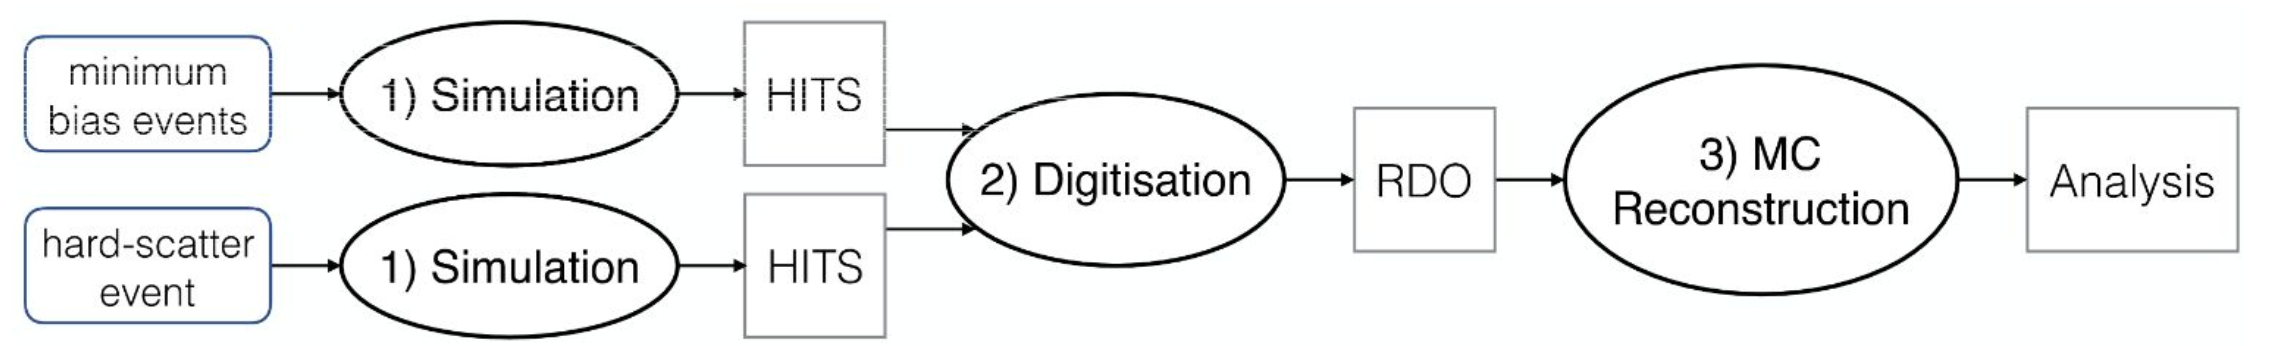
\includegraphics[width=0.9\textwidth]{Chapter2/simulation.png}
	\centering
	\begin{center}
		\caption{The full procedure of the ATLAS simulation}
		\label{Fig:simulation}            
	\end{center}
\end{figure}